\newpage
\section{Eksamensopgave 5 - Kinematik}
\begin{figure}[h!]
    \centering
    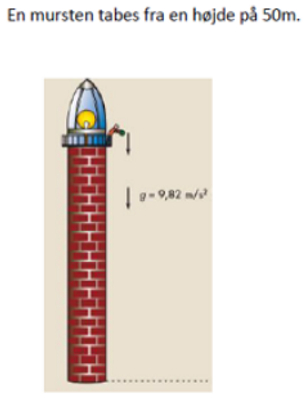
\includegraphics[width=0.3\textwidth]{figures/kinematik.png}
    \caption{Kimenatik opgave}
\end{figure}

\subsection{Diskussion}
Tager man udgangspunkt i graferne og i procent beregningerne kan man se at vores resultater har været rimelig tæt på hvad de skulle have været, inden for de 2,589\% af hvad formlen har sagt det skulle være. Vi tror at den største grund til at vi ikke er tættere er at vi ikke kan måle vinklen helt præcist og det er fordi at det er nok umuligt for et menneske at kunne gøre dette uden instrumenter der kan måle vinklen mere specifikt. Med en R2-værdi på 0,96 kan man godt sige at grafen er sikker dog er der selvfølgelig stadig usikkerhed, i dette tilfælde hvor en grad kan have stor betydning kan det dog stadig godt have en effekt at R2  ikke er tættere på 1. Hvis man kigger på det resultat vi fik til totalrefleksion kan man også se at vi var rimelig tæt på igen, 1,965\% væk fra hvad resultatet ville have været ifølge formlen. Selv om alt det her siger at vi var tætte på at ramme helt rigtigt, kan man ikke endeligt konkludere noget, da der ikke er lavet dobbelt bestemmelse.

\subsection{Konklusion}
Det kan konkluderes i det at 2 materialer mødes, skifter lyset hastighed og derved kan en brydningsvinkel bevises. Det kan derudover konkluderes, at hvis lyset kommer fra et materiale med højt brydningsindeks til et andet materiale med lavt brydningsindeks, vil alt lyset reflekteres også kendt som totalrefleksion. Det kan derfor konkluderes, at de to førnævnte formler stemmer overens med virkeligheden. Dermed er forsøgets formål opnået og kan på baggrund i rapporten. Det skal dog sige at dette ikke er et endegyldigt svar da der som nævnt i diskussionen mangler dobbeltbestemmelse og kontrolforsøg. 
\subsection{Beregn murstenens position efter 0,1s}
Først start med at identificer de kendte værdier:
\\\\
Startposition: 50 meter \newline
Start hastighed: 0 m/s (da den falder frit fra hvile position)\newline
Tid: 0,1 sekunder \newline
Tyngdeacceleration: \begin{math}9,82m/s^{2}\end{math}


\subsubsection{Brug den kinematiske formel for position}
Den generelle formel for position ved frit fald er:
\begin{equation*}
    \mathcolorbox{yellow}{s=1/2 \cdot g \cdot t^{2}}
\end{equation*}

\subsubsection{Indsæt værdierne i formlen og udregn}
\begin{equation*}
    \mathcolorbox{yellow}{1/2 \cdot 9,82m/s^{2} \cdot (0,1s)^{2}=0,0491m}
\end{equation*}

Murstenens position efter 0,1s er 49,95m

\subsection{Bestem hvor lang tid der går, inden murstenen rammer jorden}

Først identificer vi de kendte værdier som er brugt ovenover

\subsubsection{Brug den kinematiske formel for position}
\begin{equation*}
    \mathcolorbox{yellow}{1/2\cdot g\cdot t^{2}=s}
\end{equation*}
Indsæt værdierne
\begin{equation*}
    \mathcolorbox{yellow}{1/2\cdot9,82m/s^{2}\cdot t^{2}=50m}
\end{equation*}
Dette giver t = 3,191s. Hvilket betyder at der går 3,191s før murstenen rammer jorden.

\subsection{Beregn murstenens hastighed, lige inden den rammer jorden}
For at kunne udregne dett bruger vi formlen nedenunder.
\begin{equation*}
    \mathcolorbox{yellow}{v=a\cdot t}
\end{equation*}
\subsubsection{Indsæt de kendte værdier}
\begin{equation*}
    \mathcolorbox{yellow}{9,82m/s^{2}\cdot 3,191s = 31,34 m/s}
\end{equation*}


\newpage